\documentclass[12pt, letterpaper]{article}
% must use this pkg for displaying imgs
\usepackage{graphicx}
\graphicspath{ {../../imgs/} }
% pkg for links
\usepackage{hyperref}
% for codeblocks highlighting
\usepackage{listings}


\begin{document}


\newcommand{\paperauthor}{Akiel Aries}
\newcommand{\papersupervisor}{Prof. Sareh Assiri}
\newcommand{\paperuniversity}{Northern Arizona University}

\newcommand{\papertitle}{Analyzing Mirai}
\newcommand{\paperminortitle}{a *Nix-Focused Attack}
\newcommand{\papermajorheading}{Cybersecurity}
\newcommand{\paperminorheading}{CYB 410 - Software Security}

\newcommand{\HRule}{\rule{\linewidth}{0.5mm}} % Defines a new command for the horizontal lines, change thickness here

\center % Center everything on the page

%----------------------------------------------------------------------------------------
%	HEADING SECTIONS
%----------------------------------------------------------------------------------------

\textsc{\LARGE \paperuniversity}\\[1.0cm] % Name of your university/college
\textsc{\Large \papermajorheading}\\[0.2cm] % Major heading such as course name
\textsc{\large \paperminorheading}\\[0.75cm] % Minor heading such as course title

%----------------------------------------------------------------------------------------
%	TITLE SECTION
%----------------------------------------------------------------------------------------

\HRule \\[0.4cm]
{ \huge \bfseries \papertitle}\\[0.05cm] % Title of your document
{ \huge \paperminortitle}\\[0.025cm] % Title of your document
\HRule \\[3.5cm]

\begin{center}
	\makebox[0.8\textwidth]{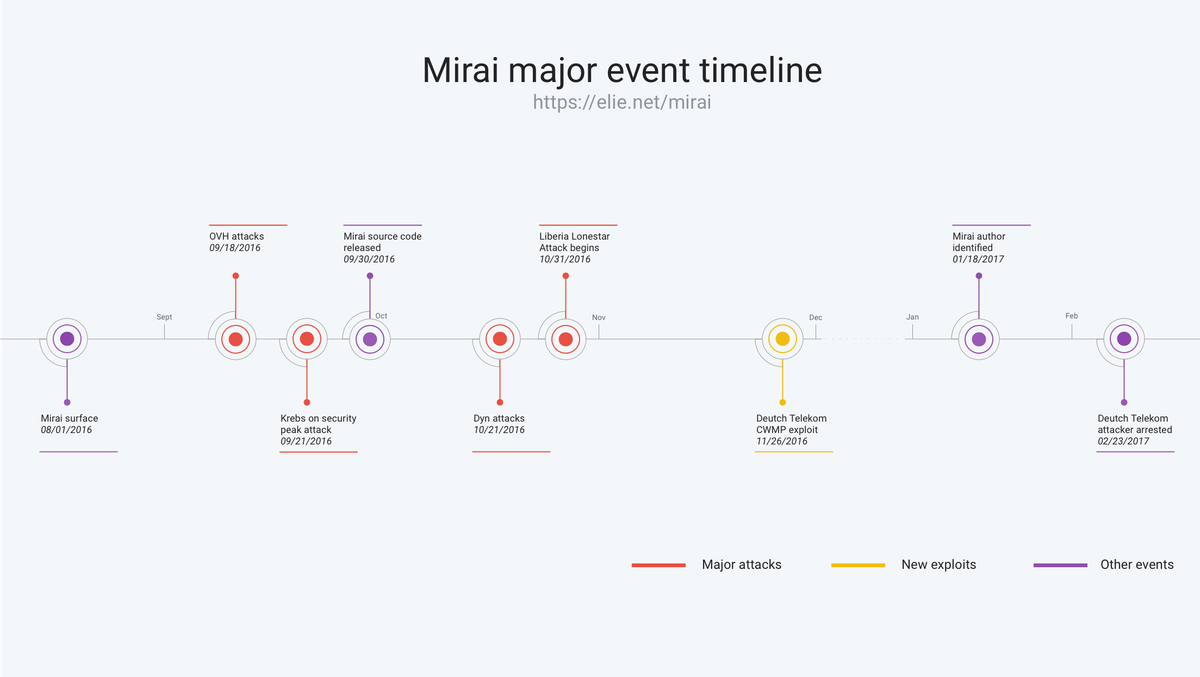
\includegraphics[width=0.8\textwidth]{mirai-major-events-timeline.png}}
\end{center}


\vfill % Fill the rest of the page with whitespace

%----------------------------------------------------------------------------------------
%	AUTHOR SECTION
%--------------------------------------------------------------------------------------

\begin{minipage}{0.4\textwidth}
	\begin{flushleft} \large
	\emph{Author:}\\
	\paperauthor
	\end{flushleft}
	\end{minipage}
	~
	\begin{minipage}{0.4\textwidth}
	\begin{flushright} \large
	\emph{Supervisor:} \\
	\papersupervisor
	\end{flushright}
\end{minipage}\\[1cm]

%----------------------------------------------------------------------------------------
%	DATE SECTION
%----------------------------------------------------------------------------------------
{\large \today}\\ % Date, change the \today to a set date if you want to be precise

\newpage

\begin{sloppypar}


% classification img
%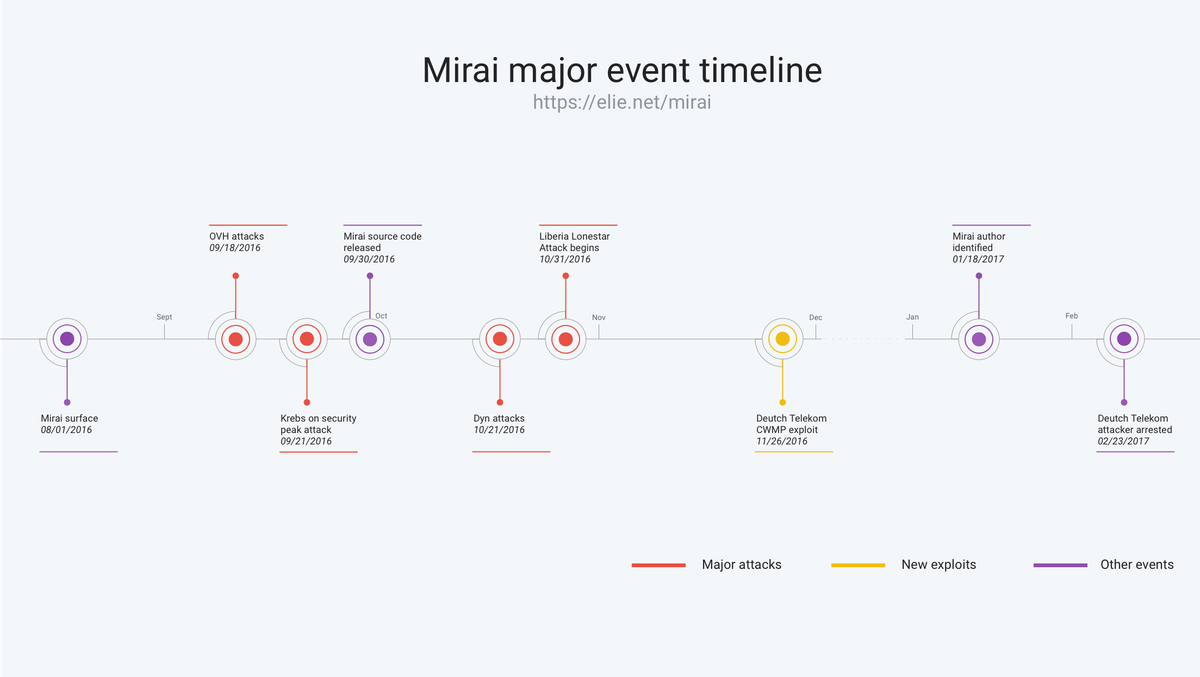
\includegraphics[scale=0.3]{mirai-major-events-timeline.png}

\section*{Introduction}
\begin{flushleft}
Mirai is a piece of malware targeting Linux based systems first discovered in 2016 by 
a malware research group MalwareMustDie and gaining more popularity when cybersecurity 
journalist, Brian Krebs, had his website attacked. The goal being to control nodes
part of a botnet running large-scale attacks. From previous research on attack history
most victims include consumer grade devices such as local home routers and IP cameras, 
which are known to be insecure and attack-prone. The bot has been used in very large-
scale DDoS (Distrubuted Denial of Service) atacks targeting many users machines and 
taking place accross the globe. Mirai's networking agent is written in C and its 
controller interface written in Go. It utilizes computer numerical control (CNC) which 
is a quite genius way to control the operation and functionality of a machine through
injection of software. Since being discover and its source code leaked, Mirai went on 
to spawn many variations, much like pieces of malware, that exploited zero-day's in 
some pieces of software for effecient and malicious operation. 


\end{flushleft}

\section*{Scale}
\begin{flushleft}
hello


\end{flushleft}


\section*{Running the Bug}
\begin{flushleft}

Requirements: \\
\begin{itemize}
\item 2 servers: 1 for CNC + mysql, 1 for scan receiver, and 1+ for loading
\end{itemize}

Setup
\begin{itemize}
\item 2 VPS and 4 servers
\item 1 VPS with extremely bulletproof host for database server
\item 1 VPS, rootkitted, for scanReceiver and distributor
\item 1 server for CNC (used like 2% CPU with 400k bots)
\item 3x 10gbps NForce servers for loading (distributor distributes to 3 servers equally)
\end{itemize}



\end{flushleft}



\section*{Static Analysis/Debugging}
\begin{flushleft}


\end{flushleft}


\section*{Final Notes}
\begin{flushleft}



\end{flushleft}


\section*{Sources}
\begin{flushleft}
https://www.imperva.com/blog/malware-analysis-mirai-ddos-botnet/
https://blog.malwaremustdie.org/2016/08/mmd-0056-2016-linuxmirai-just.html

\end{flushleft}



\end{sloppypar}
\end{document}
